Un análisis de la Universidad San Francisco de Quito (USFQ) revela que la investigación científica en Ecuador ha avanzado significativamente en los últimos 100 años, con 30.205 documentos en 27 áreas temáticas y colaboraciones de 84 países \cite{primicias2020}.


En respuesta al aumento de la producción científica y a la creciente necesidad de colaboración entre expertos, se desarrollaron dos aplicaciones que intentan abordar esta problemática, ResNet \cite{RESNET} y ResearchDecide \cite{Aimacana_2023} \cite{Padilla_2023}.

ResNet es una herramienta que utiliza modelos de minería de datos para buscar y mostrar redes de investigadores vinculados a instituciones ecuatorianas y sus áreas académicas. El objetivo principal de ResNet es representar de manera visual redes de coautoría entre investigadores ecuatorianos o investigadores que participaron en alguna publicación que tenga una afiliación ecuatoriana, utilizando datos extraídos desde Scopus \cite{SCOPUS}. El objetivo principal de ResNet es visualizar redes de coautoría entre investigadores ecuatorianos o aquellos que han participado en publicaciones con afiliaciones ecuatorianas, utilizando datos extraídos de Scopus.

Por otro lado ResearchDecide  se centra en la complejidad y la duración del proceso para lograr un consenso y la afiliación de miembros en un equipo de investigación.

En este proyecto, se propone combinar ambas plataformas para aprovechar al máximo sus funcionalidades. De esta integración nace Centinela, una aplicación robusta y capaz de abordar el problema en cuestión.

Centinela estará compuesto por cuatro componentes principales, cada uno con una función específica. Aunque cada componente puede operar de manera independiente, es fundamental que se comuniquen entre sí para su correcto funcionamiento. En la Figura \ref{fig:centinela-diagram} , se ilustra la estructura y las interacciones entre estos componentes.

\begin{figure}[H]
    \centering
    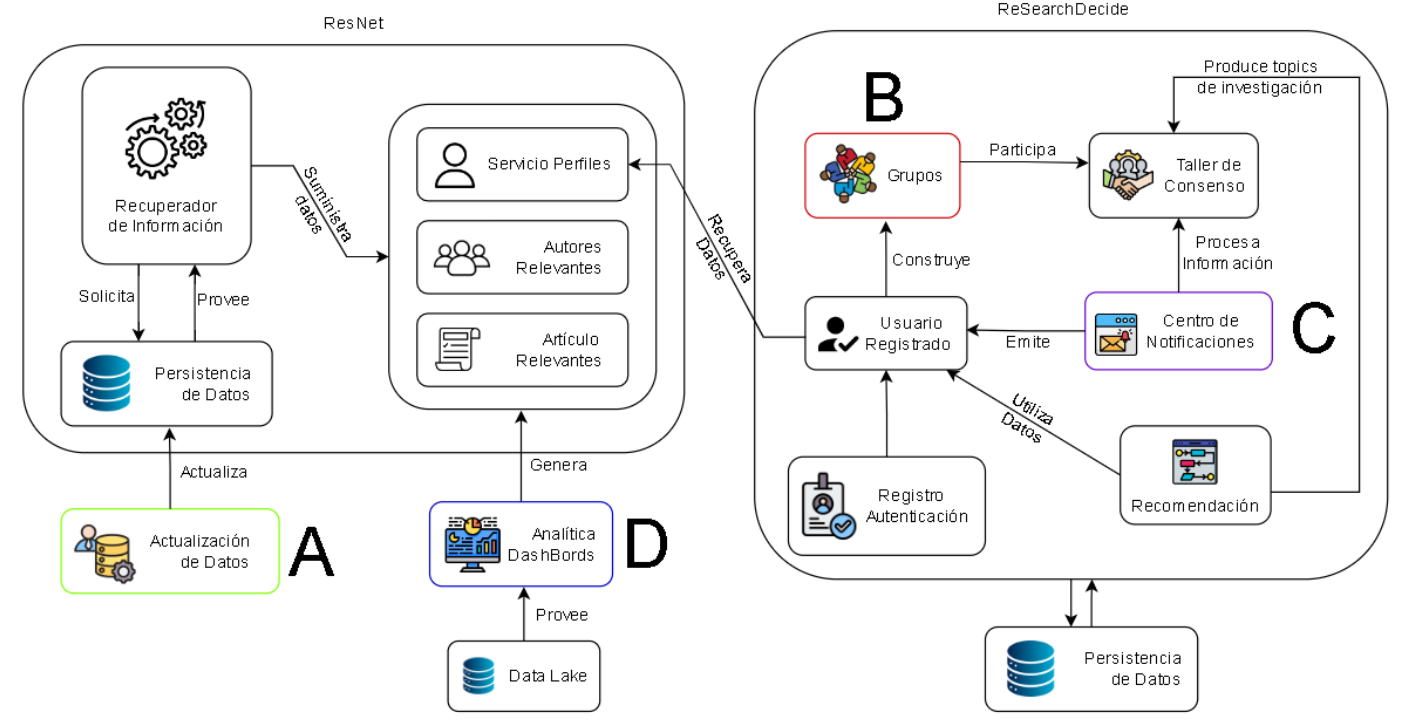
\includegraphics[scale=0.5]{../02Figures/01Chapter/centinela-architecture.png}
    \caption{Diagrama general propuesto para la integración de ResNet y ResearchDecide, mostrando la estructura y la interconexión de los componentes principales del sistema.}
    \label{fig:centinela-diagram}
\end{figure}

Debido a que actualmente en la plataforma de ResNet de extracción, limpieza y almacenamiento de datos se la hace de manera manual. Como parte del Componente A, se plantea la automatización de dicho proceso para asegurar la integridad de los datos, así como su consistencia. La automatización permitirá reducir errores humanos, aumentar la eficiencia y garantizar que los datos se manejen de manera uniforme.